\chapter{Application}
In this Chapter, the data is analyzed for cointegration relations. This will first be done pair wise by use of Engel Granger. Secondly it will be for all four simultaneously with the use of Johansen test. After the models are build, they will be used for forecasts, where the predictions will be measured against the validation data to test the precision of the models.


\section{Engel Granger Model Building}
To build the models, we first check for cointegration. This is done by making a linear model of all the $12$ possible combination of the crypto currencies. In theory cointegration is not directional, but in practice one acts as the regressand and therefore we check all $12$ combinations. Hereafter it is check whether the model is $I(0)$ which is needed for it to be cointegrated, which is done be applying the \textit{adf.test} function in \textit{R}, which calculate the augmented Dickey Fuller test, to the residuals of the model. It should be noted that the ADF's critical values are different from the normal ones used. Thus to reject the null hypothesis at a corresponding $5\%$ significance level the test statistic must be less than critical value $find hvad den skal være$. This results in the following four pair wise currencies being $I(0)$ meaning they are cointegrating. 
\pause
\begin{center}
\begin{tabular}{cccc}
   Solana \& Ethereum \quad & \quad Ripple \& Ethereum\\\\
   Ethereum \& Solana \quad & \quad Ripple \& Solana
\end{tabular}
\end{center}
\pause
\noindent The four cases will be abbreviated, SE, RE, ES and RS respectively. Next four VECM Models will be built using the above relations. First the function \textit{Varselect} is used to find the optimal lag order, the function evaluates it based on four criterions namely, Akaike Information Criterion, Hannan Quinn Criterion, Schwarz Criterion and Final prediction error. We have chosen to use AIC, since it theoretical is the best when predicting in the short term. The AIC scores for each combination have been plotted below.


\begin{figure}[!ht]
  \centering
  \subfloat[][Solana \& Ethereum]{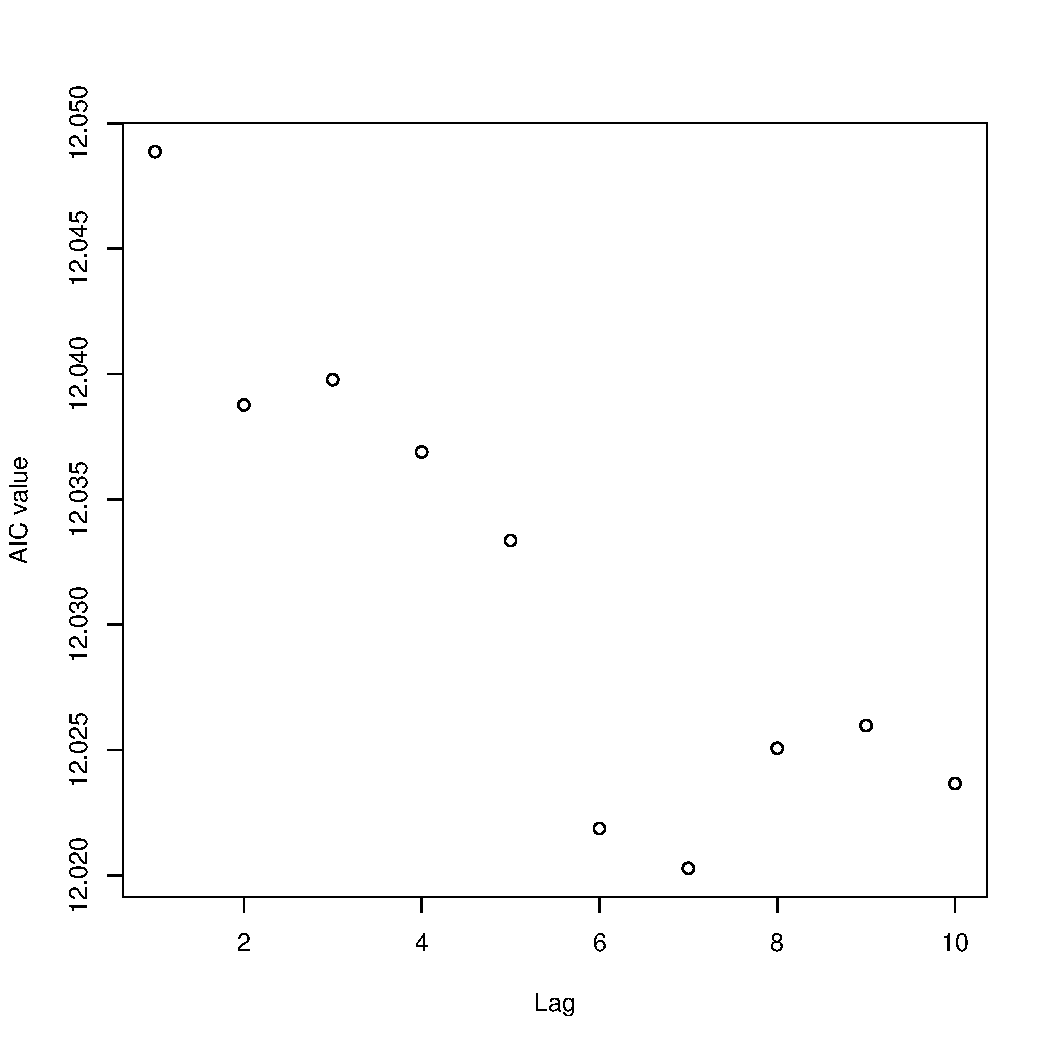
\includegraphics[width=.45\textwidth]{1.Projekt_kode/Billeder/AIC_Lag_for_SE.pdf}}\quad
  \subfloat[][Ripple \& Ethereum]{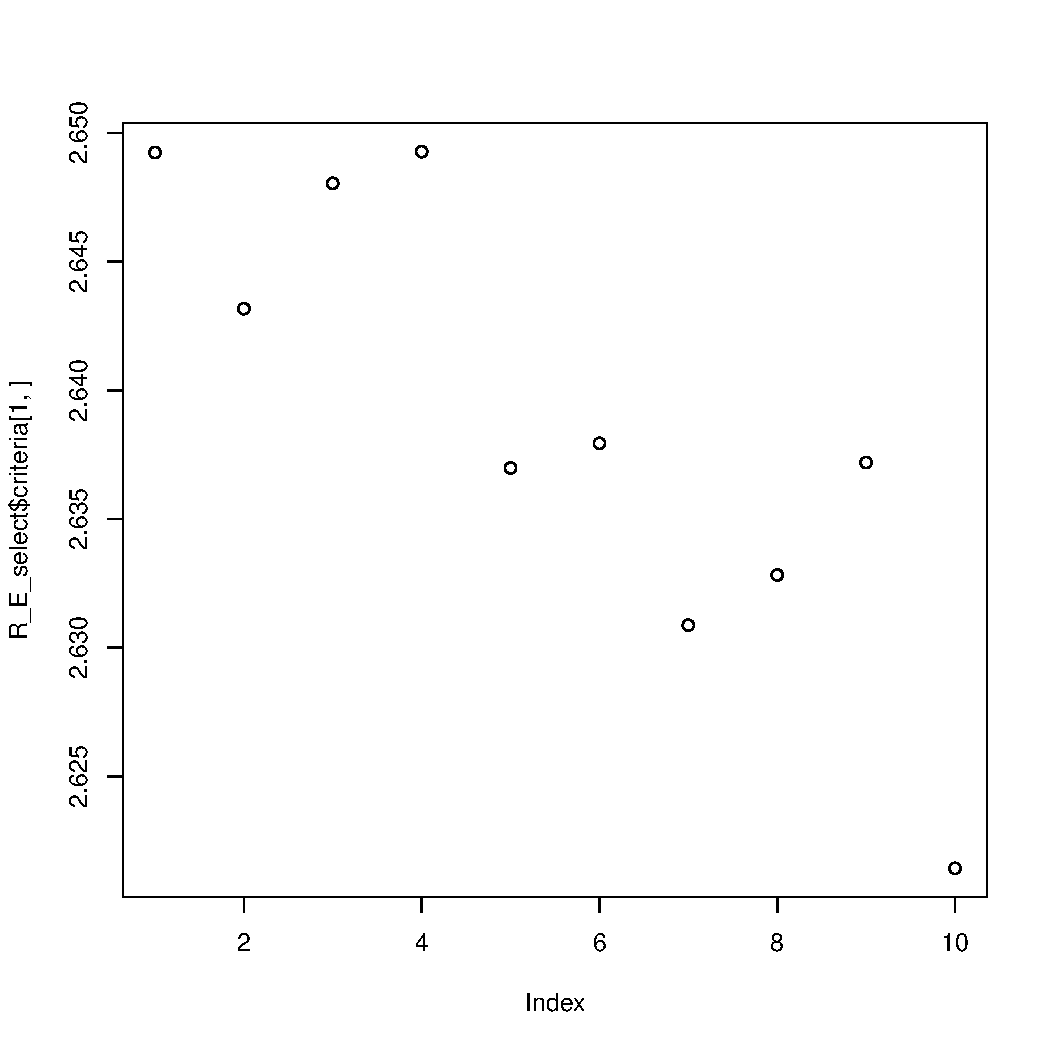
\includegraphics[width=.45\textwidth]{1.Projekt_kode/Billeder/AIC_Lag_for_RE.pdf}}\\
  \subfloat[][Ethereum \& Solana]{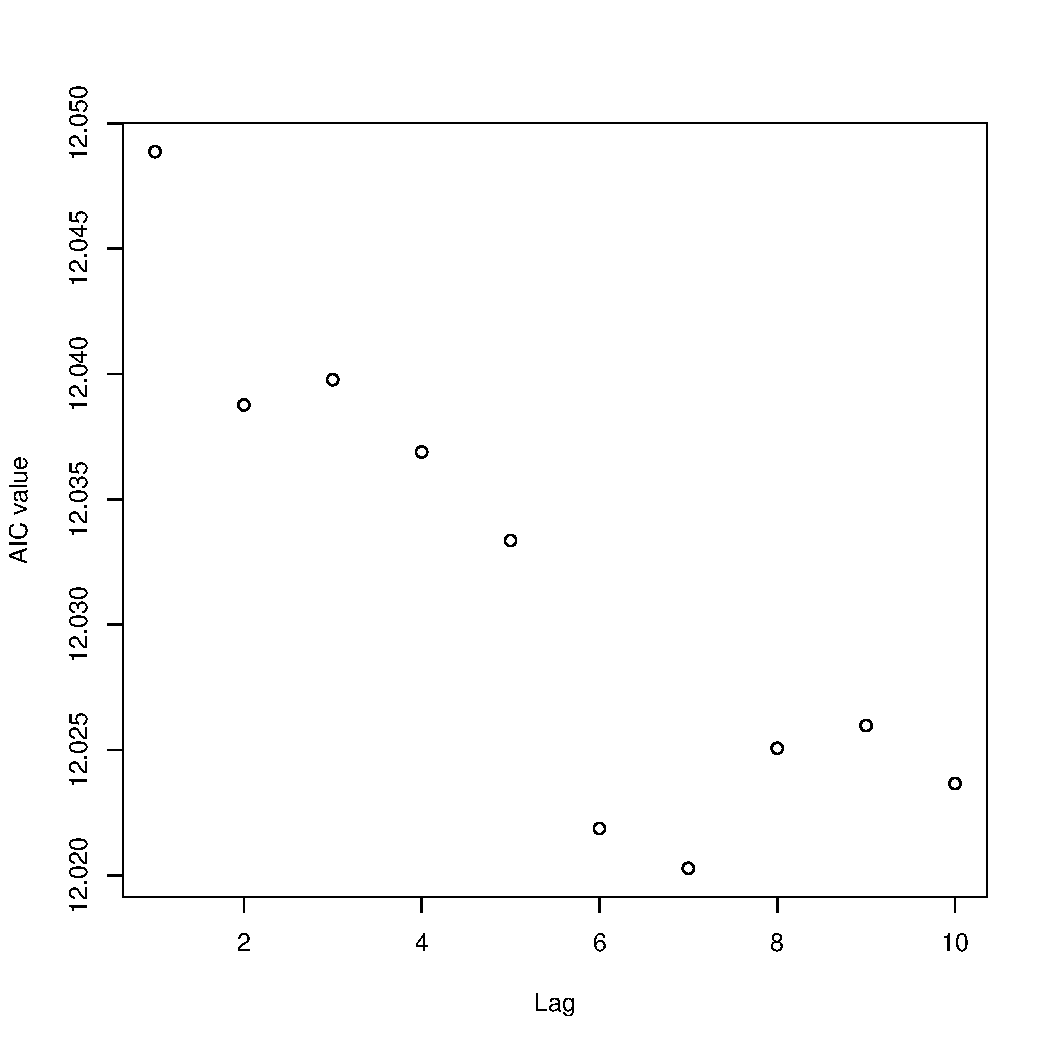
\includegraphics[width=.45\textwidth]{1.Projekt_kode/Billeder/AIC_Lag_for_ES.pdf}}\quad
  \subfloat[][Ripple \& Solana]{\includegraphics[width=.45\textwidth]{1.Projekt_kode/Billeder/AIC_Lag_for_RS.pdf}}
  \caption{AIC values for all combinations}
  \label{fig:AIC_plots}
\end{figure}

The for lags each combination are respectively . The VECM have the been made



Beta coefficients for the four models:
\begin{table}[]
    \centering
    \begin{tabular}{c|c|c}
       & SE & (1, -0.03250492) \\
       &  & 
    \end{tabular}
    \caption{Caption}
    \label{tab:my_label}
\end{table}









